 % - Components and their Interfaces
 %   - Parent subnet node
 %   - Child subnet node
 %   - IPC module
 %   - Subnet actor
 \section{Components and their Interfaces}
 \label{sec:components}

In \ipc, whole subnets need to interact.
I.e., the replicated state of one subnet must react to (changes in) the replicated state of another subnet.
As the replicated state of every subnet is distributed among its replicas and evolves independently of other subnets,
we must establish a mechanism for interactions between the states of subnets.
In particular, we must explicitly link the two replicated states of two subnets.
More precisely, for any interaction between two subnets ($A$ and $B$), define block heights $h_A$ and $h_B$,
such that $A$'s replicated state at height $h_A$ considers $B$'s replicated state to have evolved exactly until $h_B$.

To this end, we define a \emph{\pofFull (\pof)} to be data that proves that an SMR system definitively reached a certain replicated state.
Regardless of the SMR system's ordering protocol's approach to finality (e.g., immediate finality for classic BFT protocols, or probabilistic finality in PoW-based systems),
a \pof convinces the the proof's verifier that the replicated state it refers to will not be rolled back.
We denote by \emph{\pof(tx)} the proof that an SMR system reached a state in which transaction \emph{tx} already has been applied.
For example, for a BFT-based SMR system, a quorum of signatures produced by its replicas can constitute a \pof.



We separate the software needed to run \ipc into three processes and two \dapps:

\matej{\todo{Express those components and their interfaces also in pseudocode.}}
\begin{enumerate}
    \item \textbf{\ipc agent:} The software that is in charge of the interactions between the two blockchains. This includes, for example, observers for the parent and child subnets. (Note that it is a process and not a smart contract). The \ipc agent is a piece of software that mediates the interactions between the child and parent \smr software modules.    
    \item \textbf{Parent \smr replica:} The software that runs the parent blockchain. Note that this module also entails the interaction with the \ipc smart contract~\sa, which is maintained at the parent subnet. Any update that the parent process performs on \sa is notified to the \ipc agent.
    \item \textbf{Child \smr replica:} The software that runs the child blockchain. Note that some of the rules the child blockchain must satisfy are listed in~\sa. Any output operation (withdraw, checkpoint) is notified to the parent process through the \ipc agent. 
%    \item \textbf{IPC smart contract / subnet actor (\sa):} The smart contract implementation that is running on the parent blockchain. It is invoked only through transactions that are included in the parent blockchain.
    \item \textbf{IPC subnet actor (\sa):} The smart contract implementation that is running on the parent blockchain. It is invoked only through transactions that are included in the parent blockchain.
    \item \textbf{IPC coordinator/gateway actor (\gw):} a smart contract that exists in every non-leaf subnet in the \ipc hierarchy and contains methods facilitating inter-subnet operations.	
\end{enumerate}


We now define minimal interfaces between the different modules that enable the correct operation of an \ipcFull system.
A guiding principle in the interface design is to minimize changes to the \smr codebase; therefore, most extra logic of the \ipc will be added into the \ipc agent and the smart contracts \sa~and~\gw. Doing so should facilitate the deployment of \ipc with new \smr protocols by not requiring a developer familiar with \ipc to be an expert on \smr: some understanding is still needed to optimize the agent's implementation, but the \smr code would remain portable.

We require four interfaces: (i) \ipc agent --- parent \smr, (ii) \ipc agent --- child \smr, (iii) parent \smr --- \sa, and (iv) any \smr --- \gw. Both (i) and (ii) can comprise of only:
\begin{enumerate}
    \item Agent submits a transaction~\tx to the \smr process.%
    \footnote{As part of the notification defined below, it could be that after submitting \tx, until the \smr process returns \textit{complete} (perhaps with a finality parameter) or \textit{declined}, \tx is considered \textit{pending}.}
    \item Agent queries the state of the \smr process. The \smr process returns its current state (possibly limited to only a requested part of the state).
    \item \smr process notifies the agent on events of interest (e.g., changes to the state of~\sa).
\end{enumerate}

The interface between an \smr and~\sa or~\gw is based on the execution engine of that \smr and the functionality desired by~\sa. The specifics of the execution engine's system calls depend on implementation. Whenever such a call is not clear from context we provide a description of what it entails. \\


\T{The state of \sa includes representations of:}
% accounting
% Consensus functionality
% functionalities: proofOfFinality
\begin{itemize}
    \item Accounting data. This can vary from a single account representing all the parent's coins in the child to an account balance for each user in the child subnet (custodial vs non-custodial accounting). We continue with the non-custodial approach as the other can be viewed as a specific limitation of it.
    %
    \item Governance account (denoted \gov). This account facilitates the economic design of a subnet. It can be used for governing operations of the subnet. For example, collecting fees and making payments (to validators, for checkpoint reimbursement etc.) 
    %
    \item Consensus information. The data (or a pointer to it) that is needed to run the ordering of the subnet.
    \begin{itemize}
        \item Consensus protocol.
        \item Subnet configuration such as the validator set, voting rights, collateral deposits, etc.
        \item Payments methods for participation. E.g., transaction fee mechanism, block rewards.
    \end{itemize}
    %
    \item Finality verification. A method to Verify that a state/\tx is final%
    \footnote{Finality is an elusive concept that we do not take upon ourselves to define here. For simplicity, we assume finality in a Boolean manner, either \tx is final or it is not. This could easily be generalized to parameterized finality of the sort ``the probability of \tx persisting is at least~$x$."}
    in the child subnet. For this, we will use the function \sa.\verifyGfinal{\tx}{\prf} which excepts as arguments a transaction (or state) and a \prf, and outputs True if \tx is considered globally final in the child subnet and False otherwise. This function must only depend on its inputs and the internal state of~\sa. For example, \prf is a threshold signature that can be verified against the set of validators in~\sa.
  \item Parent's finality verification. A method to verify that a state/\tx is final in the parent subnet. For this, we will use the function \gw.\verifyPfinal{\tx}{\prf} which excepts as arguments a transaction (or state) and a \prf, and outputs True if \tx is considered globally final in the parent subnet and False otherwise. This function must only depend on its inputs (and perhaps some internal state of~\gw). \arp{subnet specific, not necessarily the same method for all child subnets. Lives at the SA (needed for deposits but deposits should not depend on \gw)}
\end{itemize}
%
The above suffices for an \ipcFull system with a minimal inter-subnet functionality of users' asset-transfer, and a general \smr per subnet. We continue with the additional state required for enhanced functionalities.
%
\begin{itemize}
    \item Slashing functionality.
    \begin{itemize}
        \item List of slashable misbehaviors and a proving methodology. That is, for each slashable misbehavior there is a definition of what constitutes a valid proof of misbehavior (\pom).
        \item Incentives design, i.e., specified penalties for misbehavior and rewards for reporting.
    \end{itemize}
    %
    \item Checkpointing rules.
    \begin{itemize}
        \item When checkpoints are valid. E.g., every~$\Delta$ subnet-blocks from the previous checkpoint, or the checkpoint's $L_2$ distance from the previous is larger than~$L$.
        \item Fee payments for checkpoints.
    \end{itemize}
    %
%    \item Inter-subnet transactions service (denoted \postoffice). 
%    \sa contains functionality that can be used to transfer data from one subnet to another. In particular, consider the following case involving a smart contract.%
%    \footnote{When inter-subnet data transfer happens between users (Externally Owned Accounts --- \eoa --- in Ethereum's jargon), they can actively participate in the propagation via the \ipc agent that communicates with both the parent and child subnets. Smart contracts, on the other hand, do not have that power and, therefore, cannot communicate inter-subnets as efficiently as users (\eoa).}
%    Smart contract $\textit{SmCt}$ emits an event~$e$ that contains $\textit{data}$ which is desired to reach the destination~\textit{dest} in a different subnet.
%    The \postoffice specifies the methods and the state locations that are used by this service.
\end{itemize}
Recall that \sa lives at the parent \smr. However, some of the objects that are represented in \sa are modified in the child subnet (e.g., accounting data). Therefore, such objects are likely to have a representation in the child \smr as well.
Moreover, the representation in the child \smr may differ from those in~\sa. This is due to \sa being less frequently updated (it is part of the parent \smr state). The representations are periodically synchronized, e.g., at a checkpoint event. \Cref{fig:interfaces} illustrates the components and their interfaces.\\


% We remark that all of the above are likely to have representations in the child \smr as well. Moreover, the representation in the child \smr may differ from those in~\sa. This is due to \sa being less frequently updated (it is part of the parent \smr state). The representations are periodically synchronized, e.g., at a checkpoint event. \Cref{fig:interfaces} illustrates the components and their interfaces.
\begin{figure}[h]
     \centering
     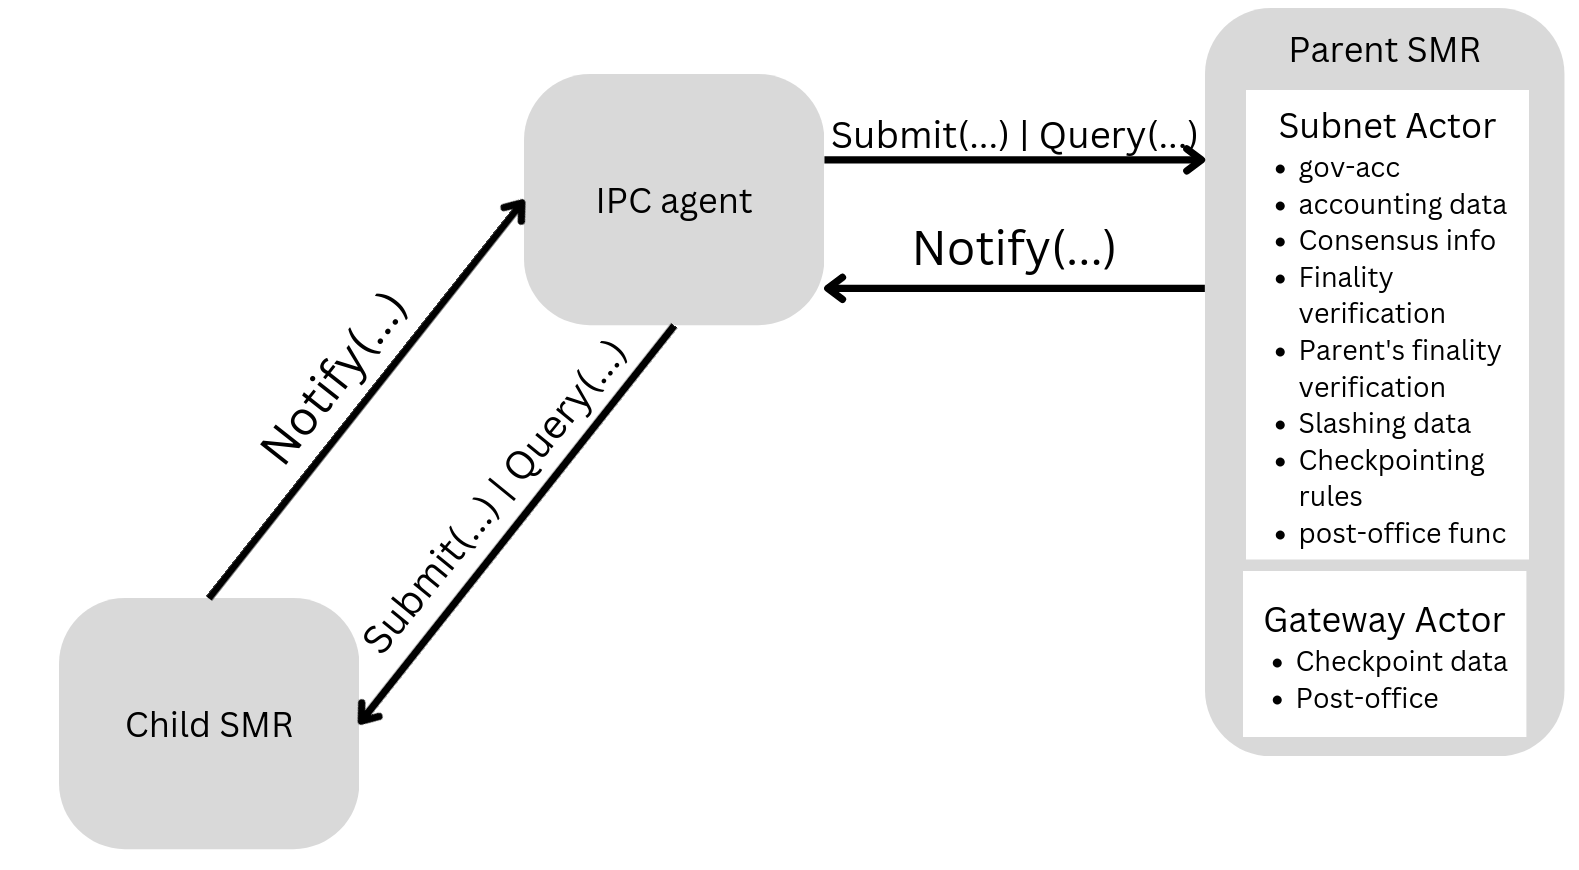
\includegraphics[width=0.75\textwidth]{compsintfs}
     \caption{The basic components and their interfaces.}
     \label{fig:interfaces}
 \end{figure}


\T{The state of \gw includes:}
\begin{itemize}
    \item Checkpoint data. The parent stores at the \gw each of the checkpoints from each direct child of it.
    \item Inter-subnet transactions service (denoted \postoffice). 
    \gw contains a registry of subnets and a functionality that can be used to transfer data from one subnet to another. 
    The \postoffice specifies the methods and the state locations that are used for these services.
    In particular, consider the following case involving a smart contract.%
    \footnote{When inter-subnet data transfer happens between users (Externally Owned Accounts --- \eoa --- in Ethereum's jargon), they can actively participate in the propagation via the \ipc agent that communicates with both the parent and child subnets. Smart contracts, on the other hand, do not have that power and, therefore, cannot communicate inter-subnets as efficiently as users (\eoa).}
    Smart contract $\textit{SmCt}$ emits an event~$e$ that contains $\textit{data}$ which is desired to reach the destination~\textit{dest} in a different subnet.
\end{itemize}
 
 
 